\documentclass[final,a0paper]{beamer}
%\documentclass[final,a1paper]{beamer}
\mode<presentation>{\usetheme{I6dv} }

\usepackage[orientation=landscape,size=a1,scale=1.8]{beamerposter}
\usepackage{exscale}
\usepackage{booktabs, array}
\usepackage[english]{babel}
\usepackage[latin1]{inputenc}
\usepackage{graphicx,color}
\usepackage{amsmath,amsthm,amssymb}
\usepackage{mpemath}
% \usepackage{algorithm}
% \usepackage{algorithmic}

\usepackage{linegoal}
\usepackage{mathtools}
\usepackage{color}
\usepackage{bm}
\usepackage[ruled,vlined,linesnumbered]{algorithm2e} %linesnumbered
\usepackage{etoolbox}

% \usepackage{algorithm}
% \usepackage{algorithmic}
%\usepackage{algpseudocode}

 \usepackage{tikz}
% \usetikzlibrary{arrows,automata}
\usepackage{graphicx}
\usetikzlibrary{arrows,decorations.markings}

\usepackage{pifont}% http://ctan.org/pkg/pifont
\newcommand{\cmark}{\ding{51}}%
\newcommand{\xmark}{\ding{55}}%

\renewcommand{\ss}{\mid}
\newcommand{\rtp}{\mathcal{P}} 
\newcommand{\rob}{^R}
% \newcommand{\tr}{^{\mathsf{T}}}
% \newcommand{\Real}{\mathbb{R}}
% \newcommand{\opt}{^\star}

% \newcommand{\E}{\mathbb{E}}
\renewcommand{\P}[1]{\mathbb{P}\left[ #1 \right]}
\newcommand{\erm}[2]{\operatorname{ERM}_{#1}\left[#2\right]}
\newcommand{\ermo}{\operatorname{ERM}}
\newcommand{\var}[2]{\operatorname{VaR}_{#1} \left[#2\right]}
\newcommand{\cvar}[2]{\operatorname{CVaR}_{#1} \left[#2\right]}
\newcommand{\evar}[2]{\operatorname{EVaR}_{#1} \left[#2\right]}
\newcommand{\vari}[2]{\operatorname{VaR}_{#1} \left[#2\right]}
\DeclareMathOperator{\kl}{KL}
\DeclareMathOperator*{\argmax}{arg\,max}
\DeclareMathOperator*{\argmin}{arg\,min}
\newcommand{\T}[0]{^{\top}} % transpose

\newcommand{\red}[1]{\textcolor{red}{#1}}
\newcommand{\blue}[1]{\textcolor{blue}{#1}}
\newcommand{\green}[1]{\textcolor{green}{#1}}
\newcommand{\cyan}[1]{\textcolor{cyan}{#1}}

\newcommand{\states}{\mathcal{S}}
\newcommand{\actions}{\mathcal{A}}

\usepackage{tikz}
\usetikzlibrary{overlay-beamer-styles}  % Overlay effects for TikZ
\usetikzlibrary{arrows,automata}

% ---- for the flow chart----
\usetikzlibrary{shapes.geometric, arrows}
\usepackage[absolute,overlay]{textpos}
\tikzstyle{startstop} = [rectangle, rounded corners, 
minimum width=2cm, 
minimum height=1cm,
text centered, 
draw=black, 
fill=red!30]

\tikzstyle{io} = [trapezium, 
trapezium stretches=true, % A later addition
trapezium left angle=70, 
trapezium right angle=110, 
minimum width=2cm, 
minimum height=1cm, text centered, 
draw=black, fill=blue!30]

\tikzstyle{process} = [rectangle, 
minimum width=3cm, 
minimum height=1cm, 
text centered, 
text width=3cm, 
draw=black, 
fill=orange!30]

\tikzstyle{decision} = [diamond, 
minimum width=3cm, 
minimum height=1cm, 
text centered, 
draw=black, 
fill=green!30]
\tikzstyle{arrow} = [thick,->,>=stealth]
% ---- for the flow chart----

\graphicspath{{fig/}}
 
\title{ROIL\@: Robust Offline Imitation Learning}
\author[]{Gersi Doko$^{1}$, Guang Yang$^{2}$, Daniel S. Brown$^{2}$, Marek Petrik$^{1}$}
\institute{$^{1}$University of New Hampshire, $^{2}$University of Utah}
  
\begin{document}
\begin{frame}{}
\vspace{-2cm}
\begin{columns}[t]
% ===== COLUMN 1 ==========
  \begin{column}{0.3\linewidth}
    \begin{block}{Summary}
\alert{Motivation}
\begin{itemize}
     \item Learning from data in a robust offline way is important in many fields, like health care, robotics or finance.
\end{itemize}
\alert{Limitations of existing  methods}
\begin{itemize}
    \item Reliance on $\hat{u}_e$ leads to covariate shift for off-policy datasets.
    \item Inability to specify reliance on $\hat{u}_e$.
    \item No guarantees of policy convergence to $u_e$ even when every state is visited.
\end{itemize}
\alert{Our contributions}
\begin{itemize}
     \item New algorithm for robust offline imitation learning.
     \item Guaranteed convergence to the optimal policy for tabular domains.
     \item Flexibility to define the reliance on $\hat{u}_e$.
\end{itemize}
\end{block}
%%% Local Variables: 
%%% mode: latex
%%% TeX-master: "main"
%%% End: 

    \begin{block}{\normalsize{Inverse Reinforcement Learning (IRL)}}
     \[
       \rho(\pi, r) = \lim_{T \to \infty} \mathbb{E}^{\pi, p_0} \lbrack \sum_{t=0}^{T} \gamma^t r(\tilde{s}_t, \pi(\tilde{s}_t)) \rbrack
     \]
     \[ 
       \pi^*_{IRL} = \argmin_{\pi \in \Pi} \max_{r \in \mathcal{R}} \rho(\hat{\pi}_e, r) - \rho(\pi, r)
     \]
     \[
       \pi^*_{ROIL} = \argmin_{\pi \in \Pi} \max_{\pi_e \in \Pi} \max_{r \in \mathcal{R}} \rho(\pi_e, r) - \rho(\pi, r)
     \]
\end{block}

%%% Local Variables: 
%%% mode: latex
%%% TeX-master: "main"
%%% End: 

    \begin{block}{\normalsize {Previous Work} }
  \begin{itemize}
  	\item \textbf{LPAL}
	\item \textbf{MILO}
	\item \textbf{GAIL}
	\item \textbf{BROIL}
  \end{itemize}
\end{block}


%%% Local Variables:
%%% mode: latex
%%% TeX-master: "poster"
%%% End:

  \end{column}
  
% ===== COLUMN 2 ==========
  \begin{column}{0.3\linewidth}
    \begin{block}{Visual Representation of ROIL}
    \begin{center}
        \begin{figure}
            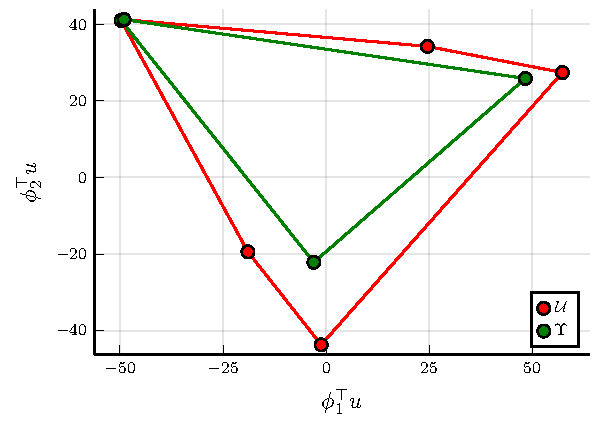
\includegraphics[width=0.85\textwidth]{../../pres_roil/plots/visual_U_and_Upsilon.pdf}
        \end{figure}
        \begin{figure}
            \begin{center}
                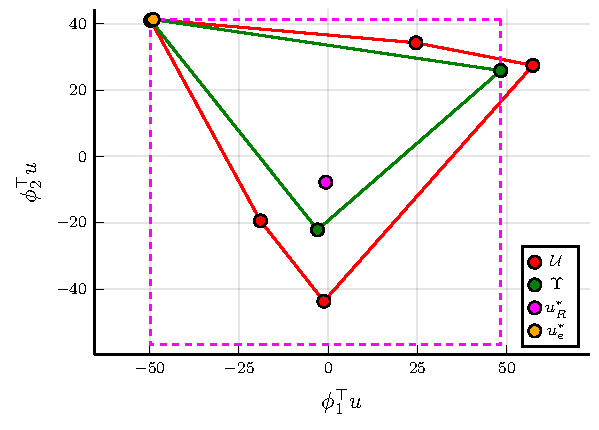
\includegraphics[width=0.85\textwidth]{../../pres_roil/plots/visual_solve_cheb.pdf}
            \end{center}
        \end{figure}
    \end{center}
\end{block}


    \begin{block}{ROIL LP}

\[ \begin{mprog}
	\minimize{t \in \Real, u \in \Real^{\mathcal{S} \times \mathcal{A}}} t
	\stc t \geq -u\tr \Phi w + \max_{v \in \Upsilon} v\tr \Phi w,\quad \forall \; w \in ext(\mathcal{W}),
        \cs u\in \Upsilon,
\end{mprog} \]

\end{block}


%%% Local Variables: 
%%% mode: latex
%%% TeX-master: "poster"
%%% End: 

  \end{column}

% ===== COLUMN 3 ==========
  \begin{column}{0.3\linewidth}
    
\begin{block}{Related Algorithms}
\begin{itemize}
    \item Prior MMDP algorithms: WSU and MVP
    \item Gradient-based MMDP methods: Mirror and Gradient
    \item Thompson sampling-based algorithms: MixTS
    \item POMDP formulations: QMDP and POMCP
\end{itemize}
% POMDP formulation and MixTS or Thompson sampling
\end{block}


\begin{block}{Simulation Results: Pest Control}
\begin{itemize}
    % \item Initialize $\pi^0$ to the WSU solution and set $\lambda_m, m \in \mathcal{M}$ to be uniform.
    % \item No additional hyper-parameters.
    \item Time horizon $T = 50$, Domain: Pest control simulation
    \item Below figure: mean returns of CADP with different initial policies. 
\end{itemize}
\begin{center}
    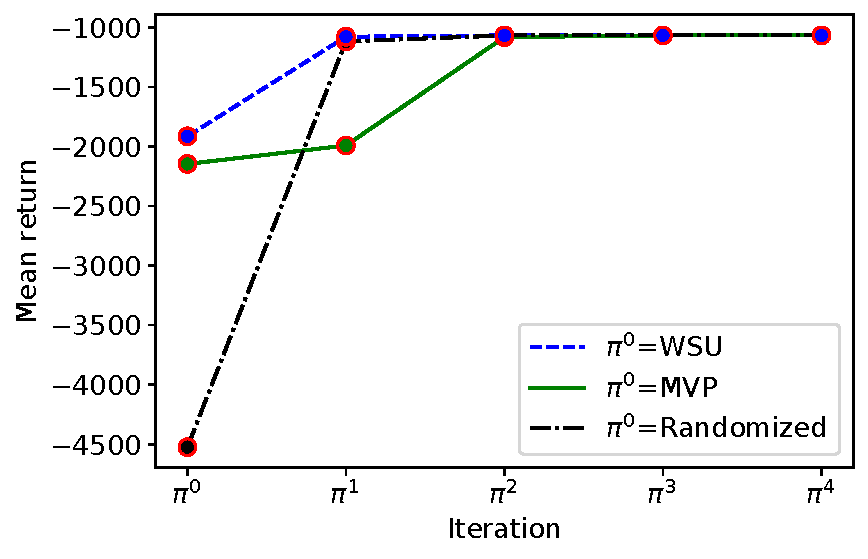
\includegraphics[width=0.6\linewidth]{fig/initial_returns.pdf}
   % Shorter the better
  \end{center}
\begin{itemize}
   \item Left figure: mean returns of algorithms, and right figure: runtimes of algorithms. 
   \item Marker X: no single policy available or runtime is greater than 900 minutes
\end{itemize}
\vspace{0.2cm}
\begin{center}
    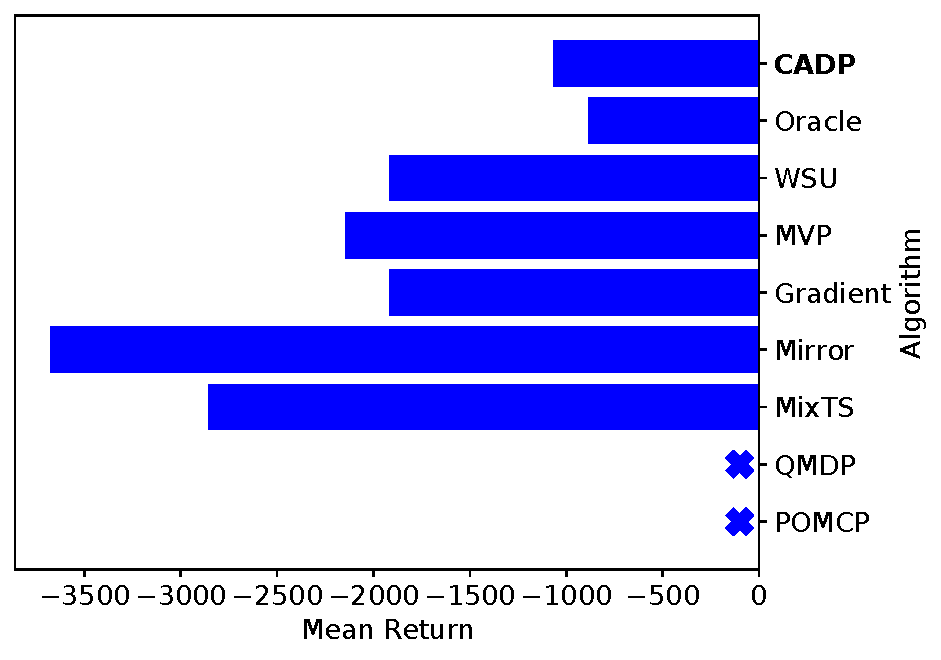
\includegraphics[width=0.49\linewidth]{fig/mean_return.pdf}
    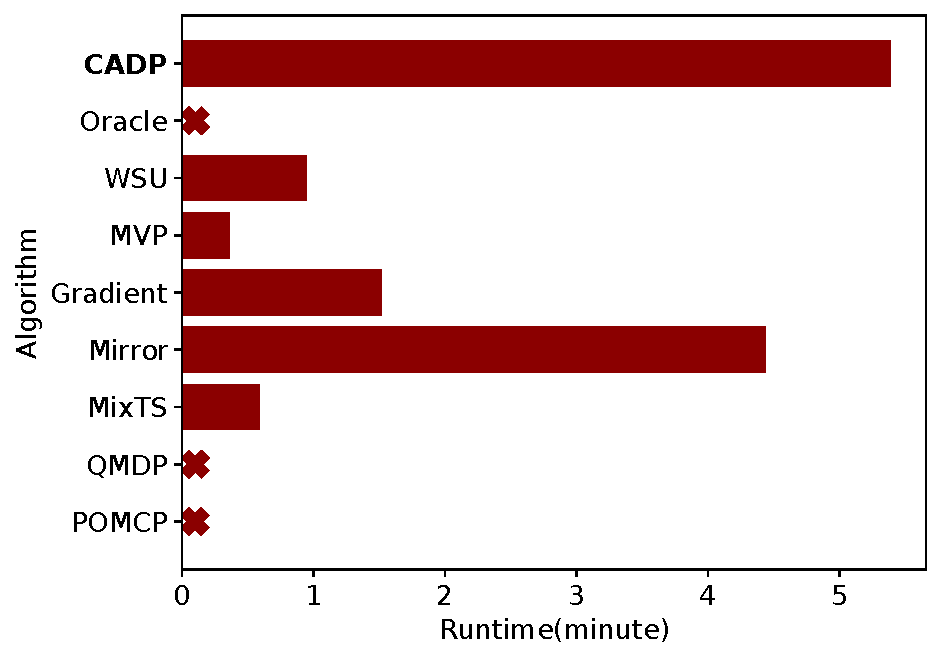
\includegraphics[width=0.49\linewidth]{fig/runtime.pdf}
  \end{center}
\end{block}
\begin{block}{Simulation Results: Other Domains}
\begin{itemize}
    \item Mean returns $\rho(\pi)$ on the test set of policies $\pi$ computed by each algorithm
\end{itemize}

 \begin{table}
    \centering
    \resizebox{\textwidth}{!}{
   \begin{tabular}{lrrrrrrrrrr}
     \toprule
     \textbf{Algorithm}  \bfseries  & \multicolumn{2}{c}{\textbf{RS}} \bfseries & \multicolumn{2}{c}{\textbf{POP}}  \bfseries & \multicolumn{2}{c}{\textbf{POPS}}\bfseries & \multicolumn{2}{c}{\textbf{INV}} & \multicolumn{2}{c}{\textbf{HIV}} \\
     \bfseries   &  T = 50  \bfseries & T =150  &  T = 50  \bfseries & T =150  &  T = 50  \bfseries & T =150  &  T = 50  \bfseries & T =150  &  T = 5  \bfseries & T =20\\
    \midrule
      \textbf{CADP}   &\textbf{204}  & \textbf{207}  & \textbf{-361} &\textbf{-368} &\textbf{-1067} &\textbf{-1082} &323 &\textbf{350} &\textbf{33348} &\textbf{42566}\\
      WSU    &203   &206  &-542     &-551   &-1915 &-1932 &323 &349   &\textbf{33348} &42564\\
      MVP    &201   &204  &-704     &-717   &-2147 &-2179 &323 &\textbf{350}  &\textbf{33348} &42564 \\ 
   \midrule
     Mirror   &181   &183  &-1650    &-1600  &-3676 &-3800 &314 &345   &\textbf{33348} &\textbf{42566}\\
    Gradient   &203   &206  &-542     &-551   &-1915 &-1932 &323 &349   &\textbf{33348} &42564\\
  \midrule
    MixTS      &167   &176  &-1761    &-1711  &-2857 &-3016 &\textbf{327} &\textbf{350}  &293 &-1026\\
    QMDP      &190   &183  & -       &-      &-     &-     &-   &-     &30705  &39626\\ 
   POMCP      &58      & 64    & -       &-      &-     &-     &-   &-     &25794  &30910\\
  \midrule
   Oracle     &210  & 213 &-168     &-172   &-882 &-894  &332 &360   &40159  &53856\\
  \bottomrule
\end{tabular}   
}
\end{table} 
	
\end{block}





  \end{column}
\end{columns}
\end{frame}
\end{document}


%%% Local Variables:
%%% mode: latex
%%% TeX-master: t
%%% End:

